\section{The audit}
\label{sec:audit}

\paragraph{Protocol.}
The audit reads two numbers from the judge's scores on the labeled set: the partial correlation with the target axis holding the nuisance axis fixed, and the reverse.
A substance-reading judge shows the first high and the second near zero; a nuisance-loaded judge shows the reverse.
Two auxiliary checks complete the instrument.
The within-correct check asks whether the judge separates sound from lucky reasoning among right answers; it must be run on the decorrelated stratum, because on the random set range restriction destroys it (the honest frontier judge reads $+0.81$ on the stratum and $-0.14$ on the random set, where $96\%$ of its scores are identical)~\cite{companionB}.
The cross-rater ceiling bounds what any signal can be credited with (Section~\ref{sec:setup}).

\subsection*{RQ1: Can the audit distinguish substance-reading from nuisance-loaded judges?}

Yes: it passes, convicts, and flips.
The honest frontier judge passes with soundness partial $+0.90$ $[+0.77, +0.97]$ and style partial $-0.22$ $[-0.40, +0.05]$ ($n{=}60$).
The sabotaged judge is convicted on the same items: style partial $+0.59$ $[+0.36, +0.76]$, soundness partial $+0.20$ $[-0.07, +0.44]$.
The audit also convicts an evaluator class it was not designed around: a top open trained reward model (Skywork-Reward-Llama-3.1-8B) scores the same traces with soundness partial $-0.01$ $[-0.29, +0.28]$ and style partial $+0.54$ $[+0.34, +0.70]$, the same signature as the sabotaged judge, where naive validation ($r = +0.18$) would report only weakness.
Under pressure the reward model shows the damage this verdict predicts: its math regret ($0.286$) is intermediate, worse than every certified referenced judge but better than every failed blind judge, and its code regret ($0.485$) is worse than every certified configuration's but below the worst blind and sabotaged code cells ($0.544$ and $0.559$).
The reward model uses no reference, so no referenced-tier comparison applies, and a single scoring function cannot supply the independent selection and reporting replicates the inflation estimand requires.
The paraphrase-replicate protocol of Section~\ref{sec:limits} supplies them: selection uses the RM's scores of the original candidates and reporting uses its scores of content-preserving Qwen-7B paraphrases of the same candidates, index-aligned, so the winner's-curse cancellation matches the judge protocol.
The registered prediction (P-R1, commit \texttt{828944a}) that the convicted reward model would show a positive excess gap larger than the certified referenced ladder's is confirmed: the measured excess gap is $+1.46\sigma$ $[+1.33, +1.58]$ ($n{=}105$; \texttt{papers/analysis/rm\_inflation.json}), the largest inflation of any configuration measured, against $+0.85$ for the sabotaged frontier, $+1.09$ for the worst blind cell (cross-family pool), and at most $+0.18$ for the certified referenced tier.
Regret is unchanged at $0.286$, because the reporting replicate does not touch selection.
The number carries a dual reading: it conflates true winner's-curse inflation with the RM's sensitivity to content-preserving rewording itself.
Both readings are damning for a deployed reward signal: either it inflates the scoreboard hardest of all evaluators measured, or its scores move by more than a sigma under paraphrase, which is presentation sensitivity by definition.
The mechanical audit of Section~\ref{sec:procedure} adds a confound to check: the reward model strongly prefers short responses (length partial $-0.54$), so part of its style conviction could be a length preference wearing style's labels, since the human style partial controls soundness but not length.
A three-variable partial answers the check directly: controlling for soundness and log response length together, the reward model's style partial moves from $+0.54$ to $+0.42$ $[+0.22, +0.59]$ and the sabotaged frontier's from $+0.59$ to $+0.47$ $[+0.26, +0.65]$, while the honest frontier is essentially unchanged ($-0.22$ to $-0.24$ $[-0.43, +0.05]$) (\texttt{papers/analysis/style\_partial\_lencontrol.json}).
Length therefore accounts for only a modest fraction of both convictions, which remain significantly positive with length controlled: the convictions are genuinely style.
An independent-annotator replication supports the honest pass and both convictions (\texttt{papers/analysis/interrater.json}).
On the 30-item subset regraded by a hypothesis-blind non-author annotator under the same rubric, the honest frontier's pattern reproduces and sharpens (soundness partial $+0.97$ on the blind rater's labels, style $-0.37$ $[-0.57, -0.08]$), and the sabotage conviction is stronger on the blind rater's labels than on the author's ($+0.61$ $[+0.30, +0.83]$ against $+0.41$ $[-0.08, +0.74]$ on this subset).
The reward-model conviction is significant on two-rater consensus ($+0.48$ $[+0.02, +0.73]$) while borderline on the blind rater's labels alone ($+0.40$ $[-0.02, +0.70]$, CI touching zero at $n{=}30$).
The verdict tracks protocol, not model identity: blind, the 1.5B judge reads style (partial $+0.51$), the 3B and 7B judges are too weak to certify, and the 14B judge clears the frozen pass rule by a hair (soundness partial $0.41$ against a $0.40$ cut), a threshold pass with no margin that Section~\ref{sec:pressure} shows to be a false pass; with the gold solution in context every honestly prompted ladder judge passes the frozen point-estimate rule (Table~\ref{tab:h2h}; the post-hoc revised rule of Section~\ref{sec:pressure} abstains on the referenced 1.5B and 3B, whose CIs straddle the bar).
A reference changes what a judge measures, not merely how accurately it measures.

\paragraph{The sabotage rubric at ladder scale, and a falsified registration.}
The two sabotaged ladder configurations (7B and 14B under the sabotage rubric) were pressure-tested early but audited only later, on the same anchor labels (\texttt{papers/analysis/sabotage\_ladder\_audit.json}).
Their audit runs were registered pre-run at pipeline commit \texttt{718c399} with the prediction that both would be convicted.
That registered prediction is falsified: neither style partial is significantly positive (7B $+0.17$ $[-0.06, +0.38]$; 14B $+0.24$ $[-0.07, +0.47]$), so under the frozen rule neither is convicted.
Both instead fail, with soundness partials $+0.28$ $[+0.07, +0.46]$ and $+0.38$ $[+0.06, +0.62]$ below the $0.40$ cut.
Both fail verdicts are correct predictions: under pressure both configurations land in the failed cluster (regrets $0.400$ and $0.324$).
Because the verdict-versus-outcome scoring happened after the pressure outcomes were known, these two rows enter the accounting as confirmatory additions rather than registered-era predictions (Appendix~\ref{app:confusion}).
The scale comparison carries a mechanism: the sabotage instruction loads style only at frontier capability (style partial $+0.59$ at GPT-5.2 against $+0.17$ and $+0.24$ at 7B and 14B, both ladder CIs crossing zero), while at ladder scale it instead degrades the judge into a weak one (soundness partials fall to $+0.28$ and $+0.38$ from the honest referenced $+0.66$ and $+0.70$).
Corrupt instructions are therefore capability-gated, which strengthens the case that the audit must run per deployment rather than per model class.

\begin{figure}[t]
\centering
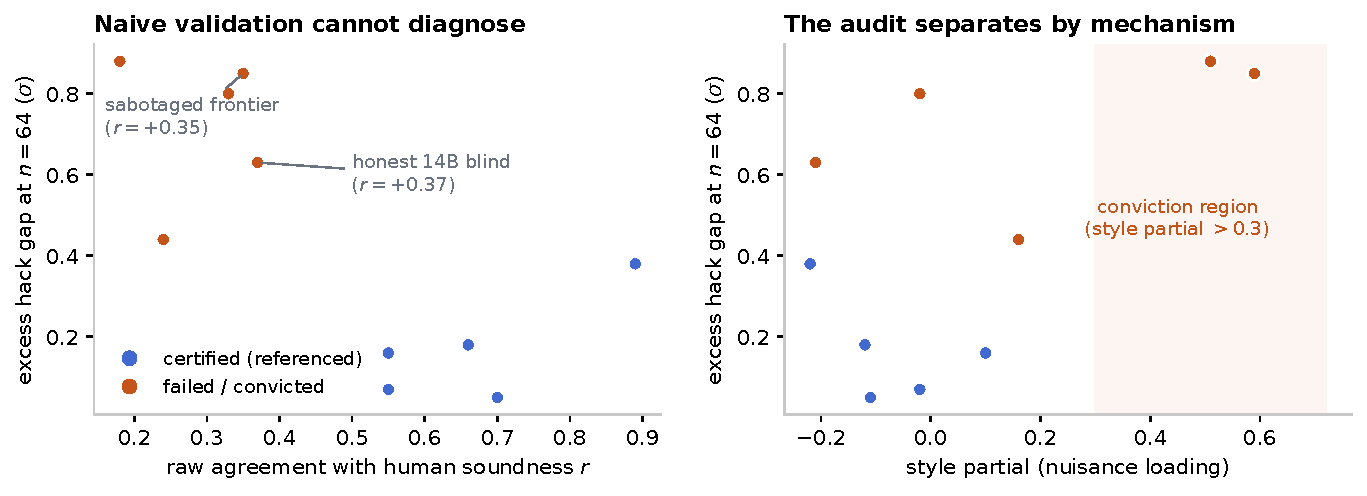
\includegraphics[width=\textwidth]{figures/fig_h2h.pdf}
\caption{\textbf{The head-to-head, visualized.}
Each point is one audited math configuration; the $y$ axis is its scoreboard inflation under best-of-64 pressure.
Left: raw agreement with human soundness places the sabotaged frontier judge inside the failed-blind cluster.
Right: the style partial isolates both style-loaded configurations in a sign-anchored conviction region fixed before outcomes.
\textbf{Takeaway: naive validation ranks but cannot diagnose; the audit's nuisance axis separates capable-corrupt from weak-honest.}}
\label{fig:h2h}
\end{figure}

\subsection*{RQ2: Does raw human agreement suffice instead?}

No, and Table~\ref{tab:h2h} and Figure~\ref{fig:h2h} locate the two failures precisely.
Raw agreement is not useless: referenced judges score higher than blind ones, and a threshold placed between the clusters would have called the ladder outcomes.
It fails first by conflating weak-honest with capable-corrupt, the distinction that determines the failure mode under pressure.
It fails second by offering no principled threshold: the separating value is knowable only after the outcomes.
The audit shares the threshold problem for its weak-judge boundary (the 3B-blind partials straddle zero within noise, and the 14B-blind false pass of Section~\ref{sec:pressure} is that problem realized), but its convictions do not: a significantly positive nuisance partial is a sign condition, fixed ex ante, and it alone identifies both style-loaded configurations.
The audit's advantage is diagnosis and sign-anchored conviction, not a magically sharper threshold for weak judges.

\paragraph{Incremental validity over a protocol bit.}
The strongest trivial baseline is a protocol-bit classifier that predicts certified behavior iff a reference is present.
On the same thirteen configurations it scores ten of thirteen: it is wrong on all three sabotaged referenced arms, which it cannot see, and right on the blind 14B, where the audit false-passes.
The audit scores twelve of thirteen.
The audit's incremental value is precisely detection of corrupted instructions and reward models that protocol bits cannot see, at the cost of one boundary miss.

\paragraph{Multiple comparisons.}
The conviction rule is a single pre-declared sign condition per configuration, a significantly positive nuisance partial, not a search over thresholds, which bounds the multiplicity concern.
A Bonferroni correction across the eleven registered-era audited configurations leaves all three convictions significant: recomputing the style-partial bootstrap CIs at the corrected level keeps them wide of zero (sabotaged frontier $[+0.25, +0.80]$, reward model $[+0.20, +0.77]$), and the 1.5B-blind conviction's permutation test gives $p = 0.0017$ (two-sided, $n{=}53$), below the corrected level $0.05/11$ (corrected conviction CIs in \texttt{papers/analysis/conviction\_bonferroni.json}).

\paragraph{Verdict stability.}
Convictions and strong passes stabilize with the fewest labels.
At 40 labels, the sabotage conviction and the honest frontier pass reproduce in $100\%$ of label resamples, while boundary configurations (the 1.5B referenced pass, the 14B blind threshold pass that Section~\ref{sec:pressure} shows to be false) remain unstable at $50$ labels and below (the 14B blind verdict reproduces fully only at the complete $60$-label set; the 1.5B referenced pass reaches $94\%$ at $50$ of its $56$ labels) (Figure~\ref{fig:stability}).
A few dozen labels certify clear cases; boundary verdicts honestly demand more.

\begin{figure}[t]
\centering
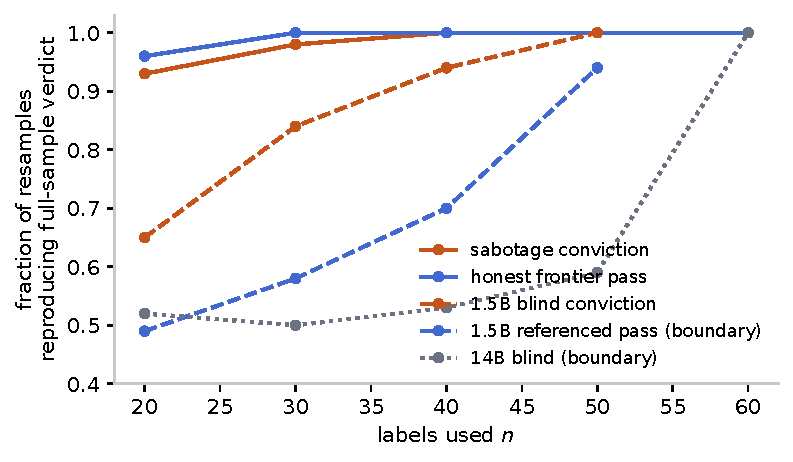
\includegraphics[width=0.62\textwidth]{figures/fig_stability.pdf}
\caption{\textbf{Verdict stability under label subsampling} (500 resamples per point, fixed verdict rules).
\textbf{Takeaway: convictions are cheap and stable; verdicts near the pass boundary are the ones that need more labels.}}
\label{fig:stability}
\end{figure}

\paragraph{What the certificate covers: outcomes, not process.}
Even certified judges grade endpoints rather than checking each line.
With planted errors whose wrong value propagates coherently to the final answer, frontier judges catch essentially all; with planted false steps that do not change the final answer, they forgive $40$--$50\%$~\cite{companionB}.
A pass therefore certifies soundness-tracking at the solution level, not step-level process verification.

\paragraph{A zero-label pre-screen.}
An order-swap test costs nothing: ask the same pairwise comparison twice with the order flipped and measure the flip rate.
Across the ladder the flip rate falls from $71$--$95\%$ at 0.5B to $2$--$37\%$ at 14B~\cite{companionB}.
A judge that cannot agree with itself under order swap cannot pass any validity audit, so the free tier eliminates hopeless judges and reserves labels for certifiable ones.

\paragraph{When a reference helps.}
On planted-error detection, the ladder detects $3/17/49/75\%$ of errors blind and $21/85/85/90\%$ with the gold reference; the 3B jump replicates in six model families ($+14$ to $+60$ points)~\cite{companionB}.
Producing a reference is the hard part, not using one: a judge that first solves the problem and then grades against its own solution detects $59/60/85/95\%$, above gold at 1.5B and 14B, matching at 7B, trailing at 3B.
Part of small-judge weakness is protocol, not capability.

\paragraph{When a reference hurts.}
On tasks with many valid answers the reference lever inverts, statically and dynamically.
Statically, any reference, whoever wrote it, costs $7$--$8$ points of verdict accuracy (paired, $p \le .0005$)~\cite{companionD}.
Dynamically, under best-of-64 pressure on multi-valid tasks, the referenced judge is more inflated than the blind one at all four ladder sizes (for example 3B: gap $+0.55$ blind versus $+1.21$ referenced), and the mechanism is directly measurable: among equally valid answers, referenced judges score those matching the shown reference $+2.7$ to $+10.0$ points (of 10) above the rest, with total anchoring at 1.5B--3B, while blind judges show no such margin~\cite{companionD}.
A reference converts a judge into a verifier only when the task's answer is effectively unique and checking against the reference is within the judge's capability.
